%!TEX root = ../main.tex

\chapter{Camera calibration\label{chap:calib}}

For the correct representation of distances and angles in the received data from the camera, a camera calibration with the used lenses needs to be performed.
The lenses used to obtain the data were a 2.5mm f/1.6 fisheye lens, with a $187$ degrees \ac{FOV} and Entaniya 1.07mm f/2.8 fish eye lens with a FOV 
of $280$ degrees, both can be seen in \reffig{fig:lenses}.
%\begin{figure}[H]
%  \centering
%  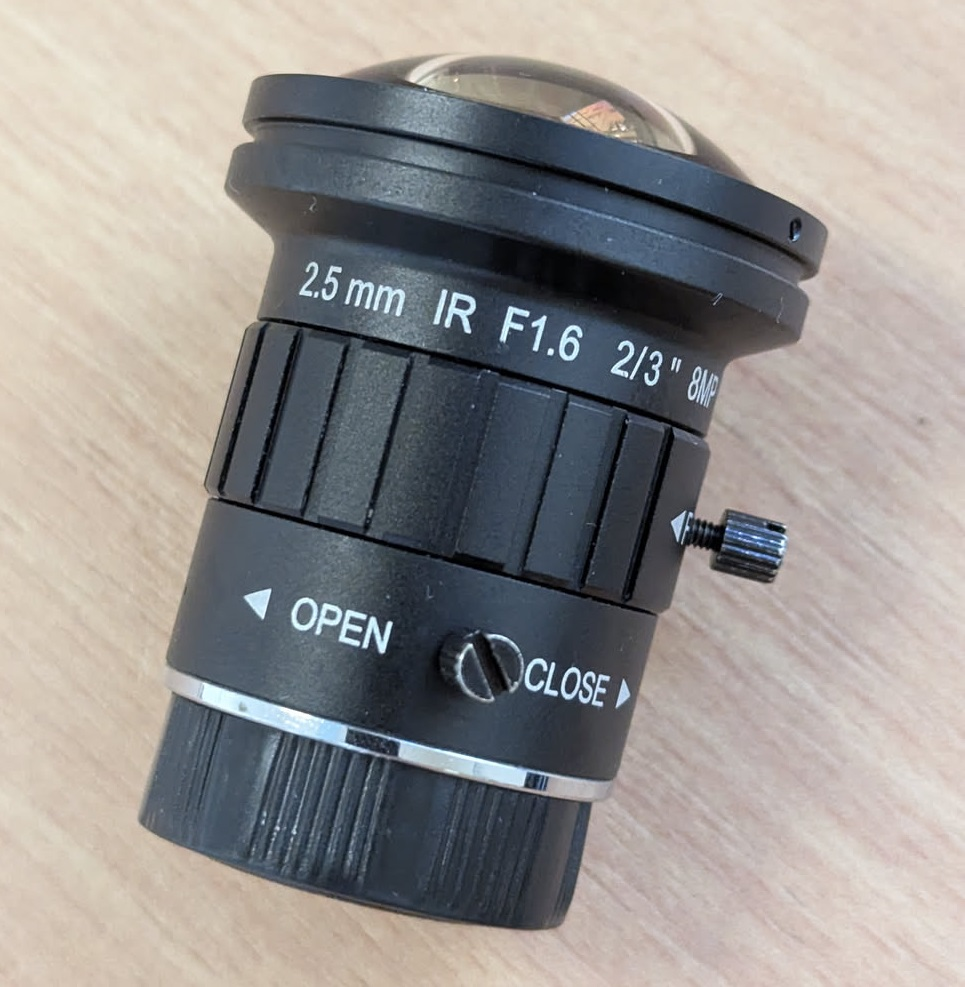
\includegraphics[width=0.5\textwidth]{./fig/photos/lens.jpeg}
%  \caption{2.5mm f/1.6 fish eye lens.}
%  \label{fig:fisheye_lens}
%\end{figure}

\begin{figure}[H]
	\centering
	\subfloat[2.5mm f/1.6 fish eye lens] {
	  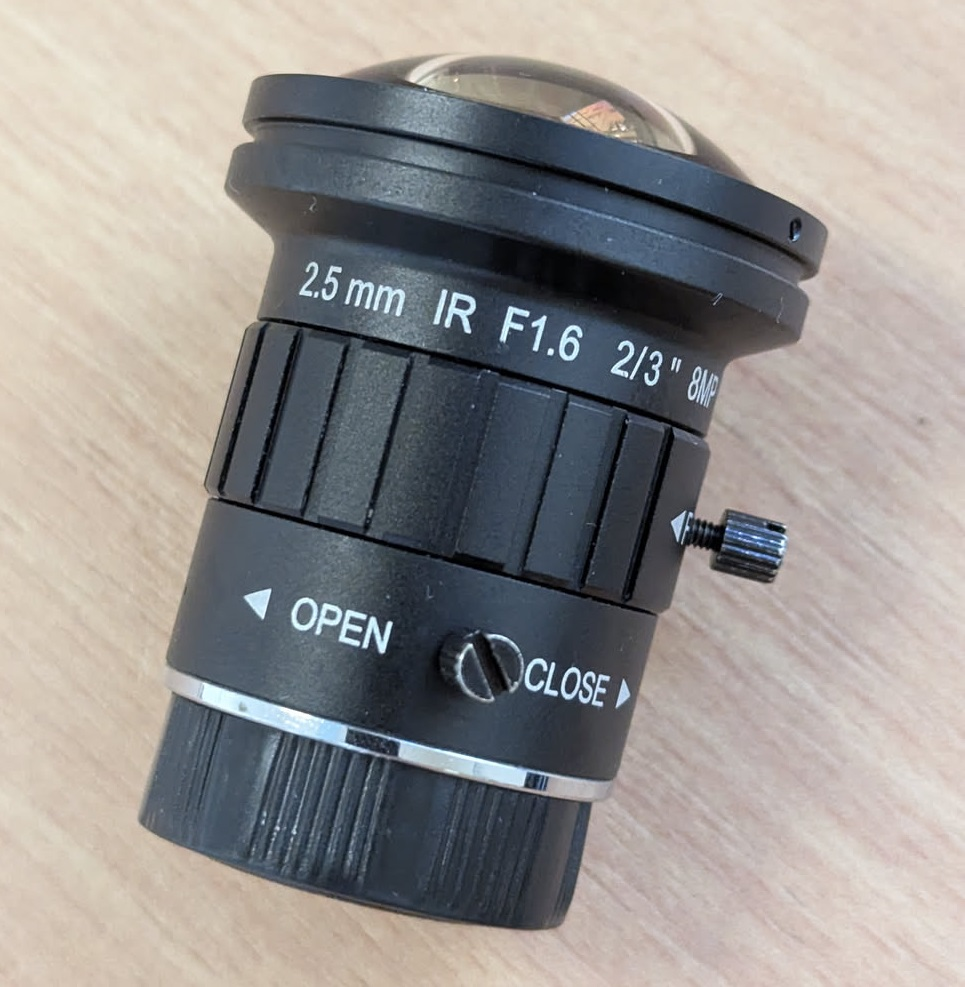
\includegraphics[width=0.4\textwidth]{./fig/photos/lens.jpeg}
	  \label{fig:lens_1}
	}
	\subfloat[1.07mm f/2.8 Entaniya fish eye lens] {
	  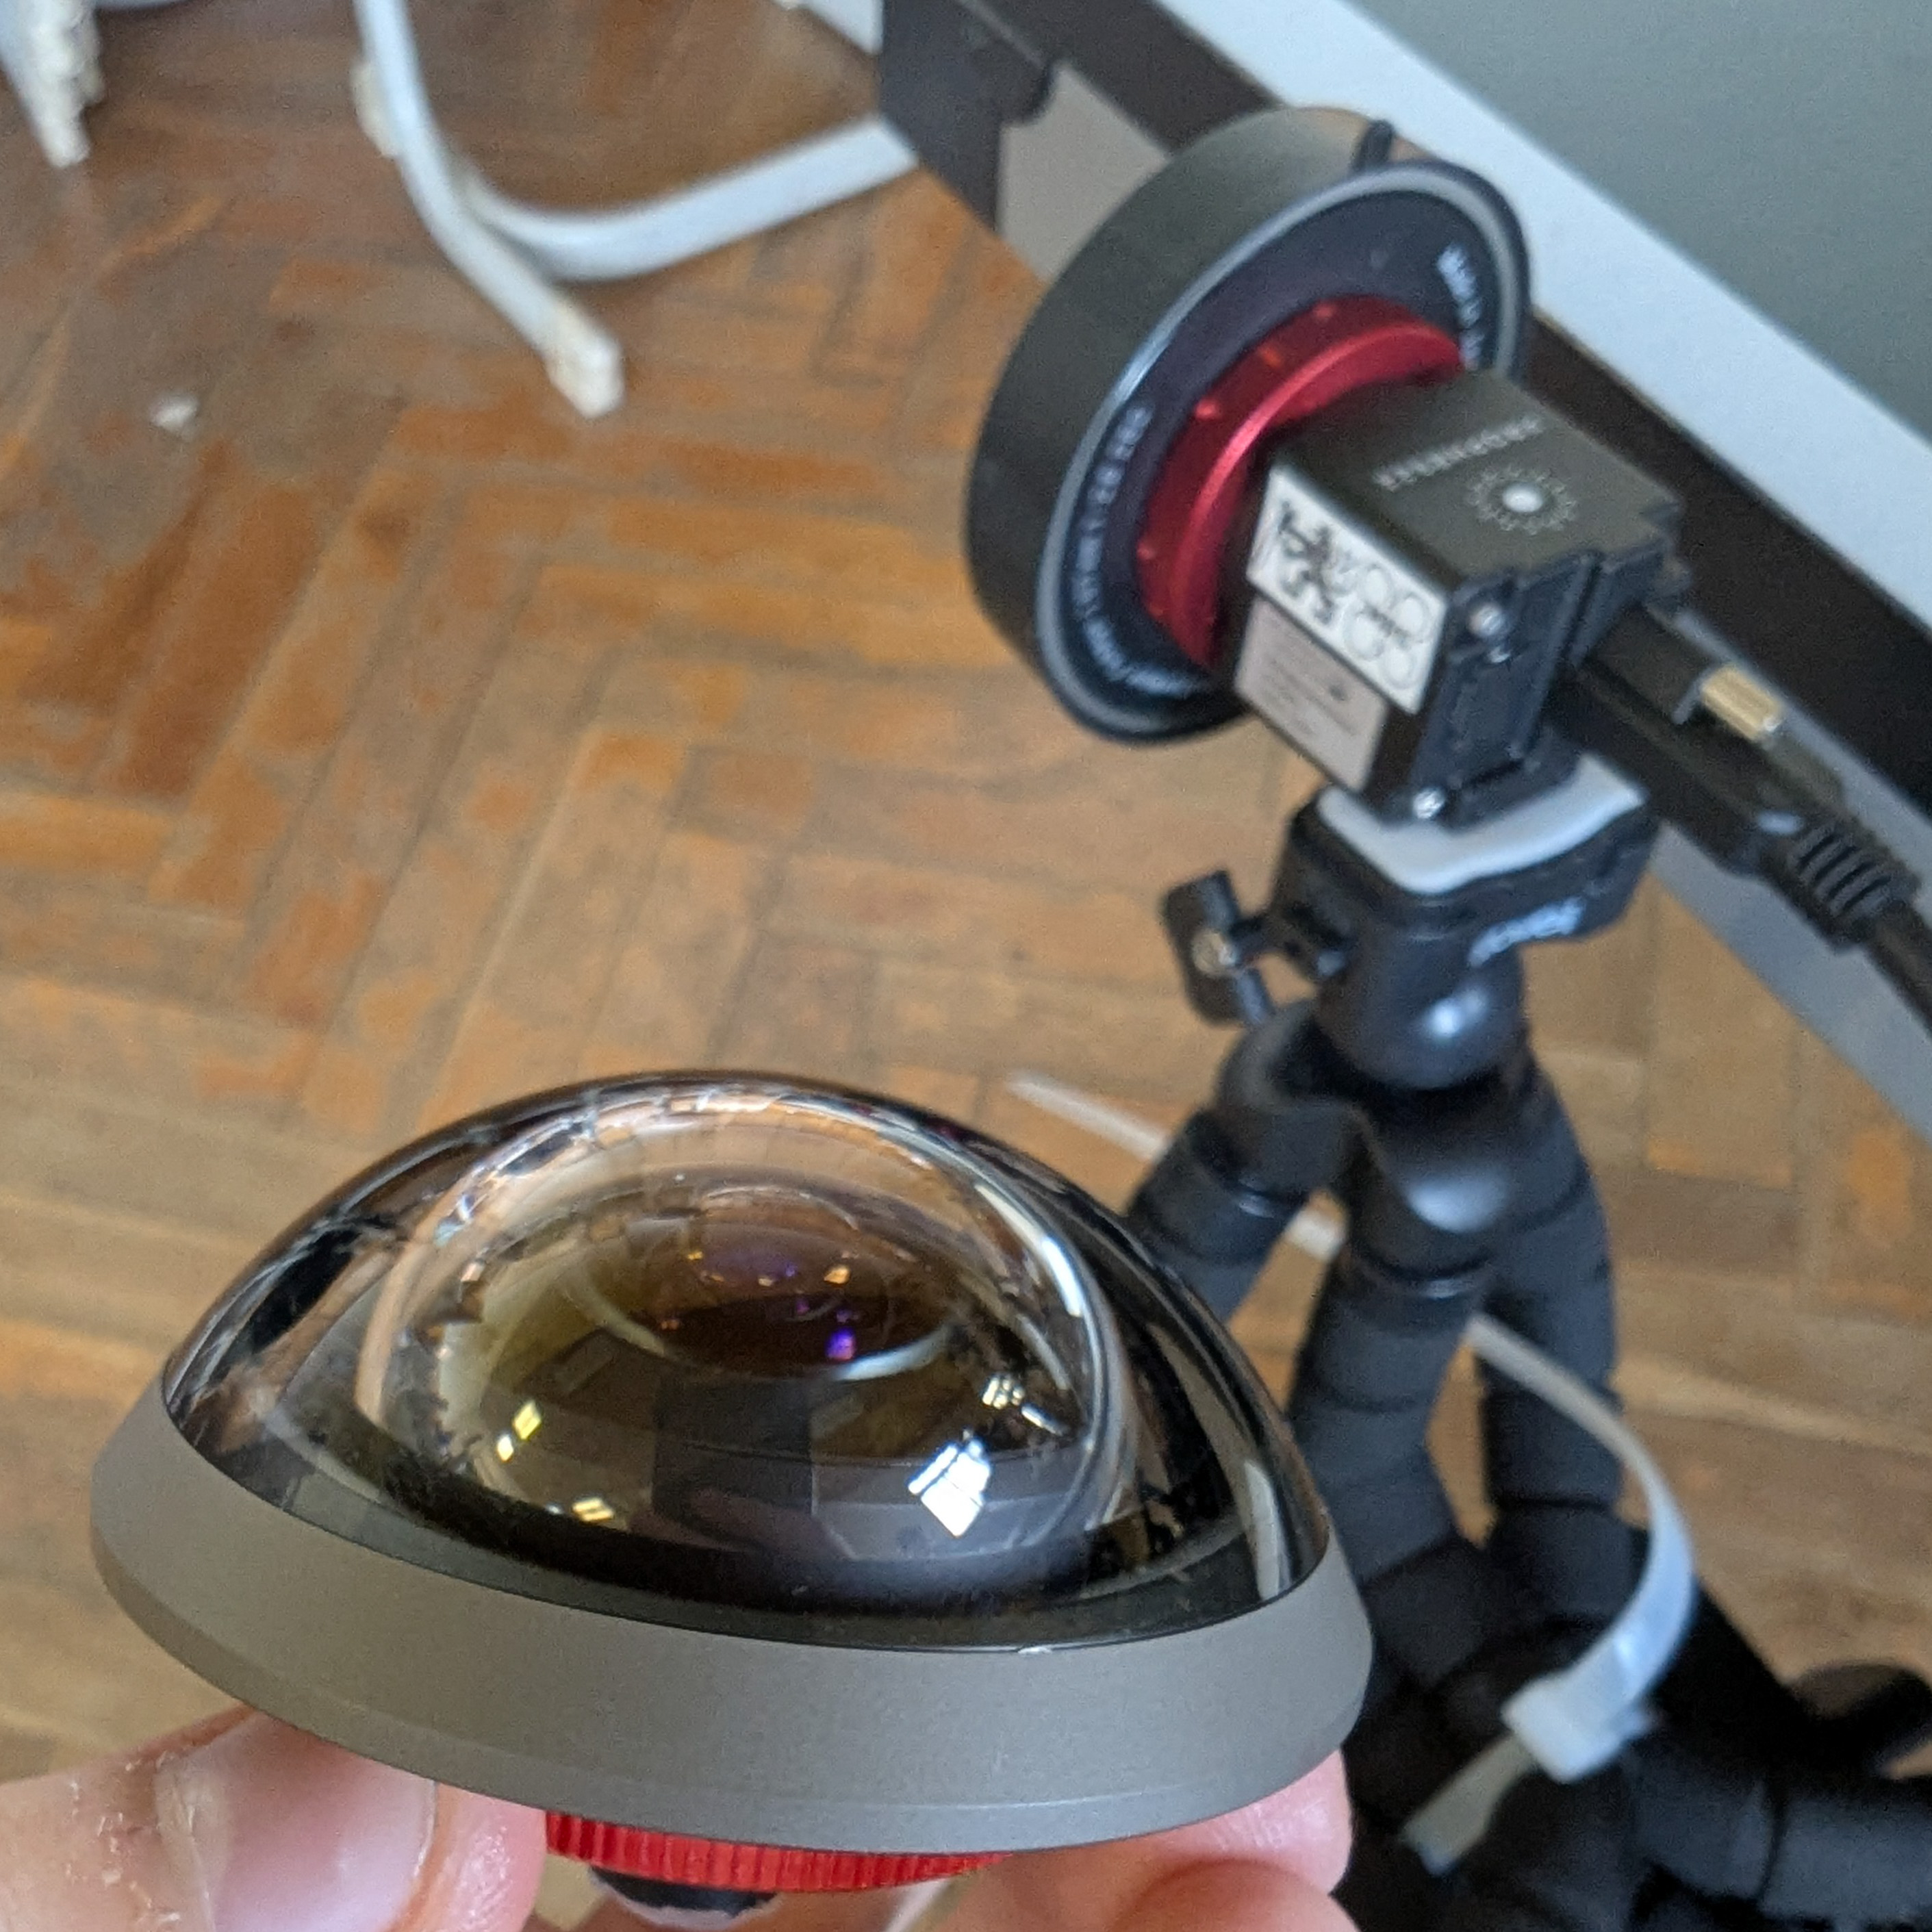
\includegraphics[width=0.4\textwidth]{./fig/photos/entaniya_280.jpg}
	  \label{fig:lens_2}
	}
	\caption{
		Lenses used during the calibration, a $187$ degree lens in \reffig{fig:lens_1} and Entaniya $280$ degree lens in \reffig{fig:lens_2}.
  }
	\label{fig:lenses}
\end{figure}

\section{Method used}

In this work a calibration method proposed by Scaramuzza et al. \cite{scaramuzzacalibration} for omnidirectional camera calibration is used to calibrate all the equipment used. The implementation used for calibration is a Python library \texttt{py-OCamCalib} \footnote{\texttt{py-OCamCalib} is available at \url{https://github.com/jakarto3d/py-OCamCalib}}.%TODO: maybe cite the github repo
For calibration purposes, a calibration chessboard pattern is usually used, which offers high contrast between squares (and thus easy detections of square corners) and
a known square size. Multiple images are usually taken, at various rotations and distances, to obtain good calibration results.
In our calibration procedure, we use a $5\times7$ lattice of UV LEDs, which are spaced 50 mm apart from each other. With this pattern, events are generated at the center of the
LEDs and can be detected by any kind of blob detector. The LED lattice is used, so the event camera can easily detect events from bright LEDs, as opposed to
the light being reflected from the chessboard pattern (which does not produce any light on its own).
The calibration lattice can be seen in \reffig{fig:lattice}.

\begin{figure}[H]
	\centering
	\subfloat[Calibration lattice] {
	  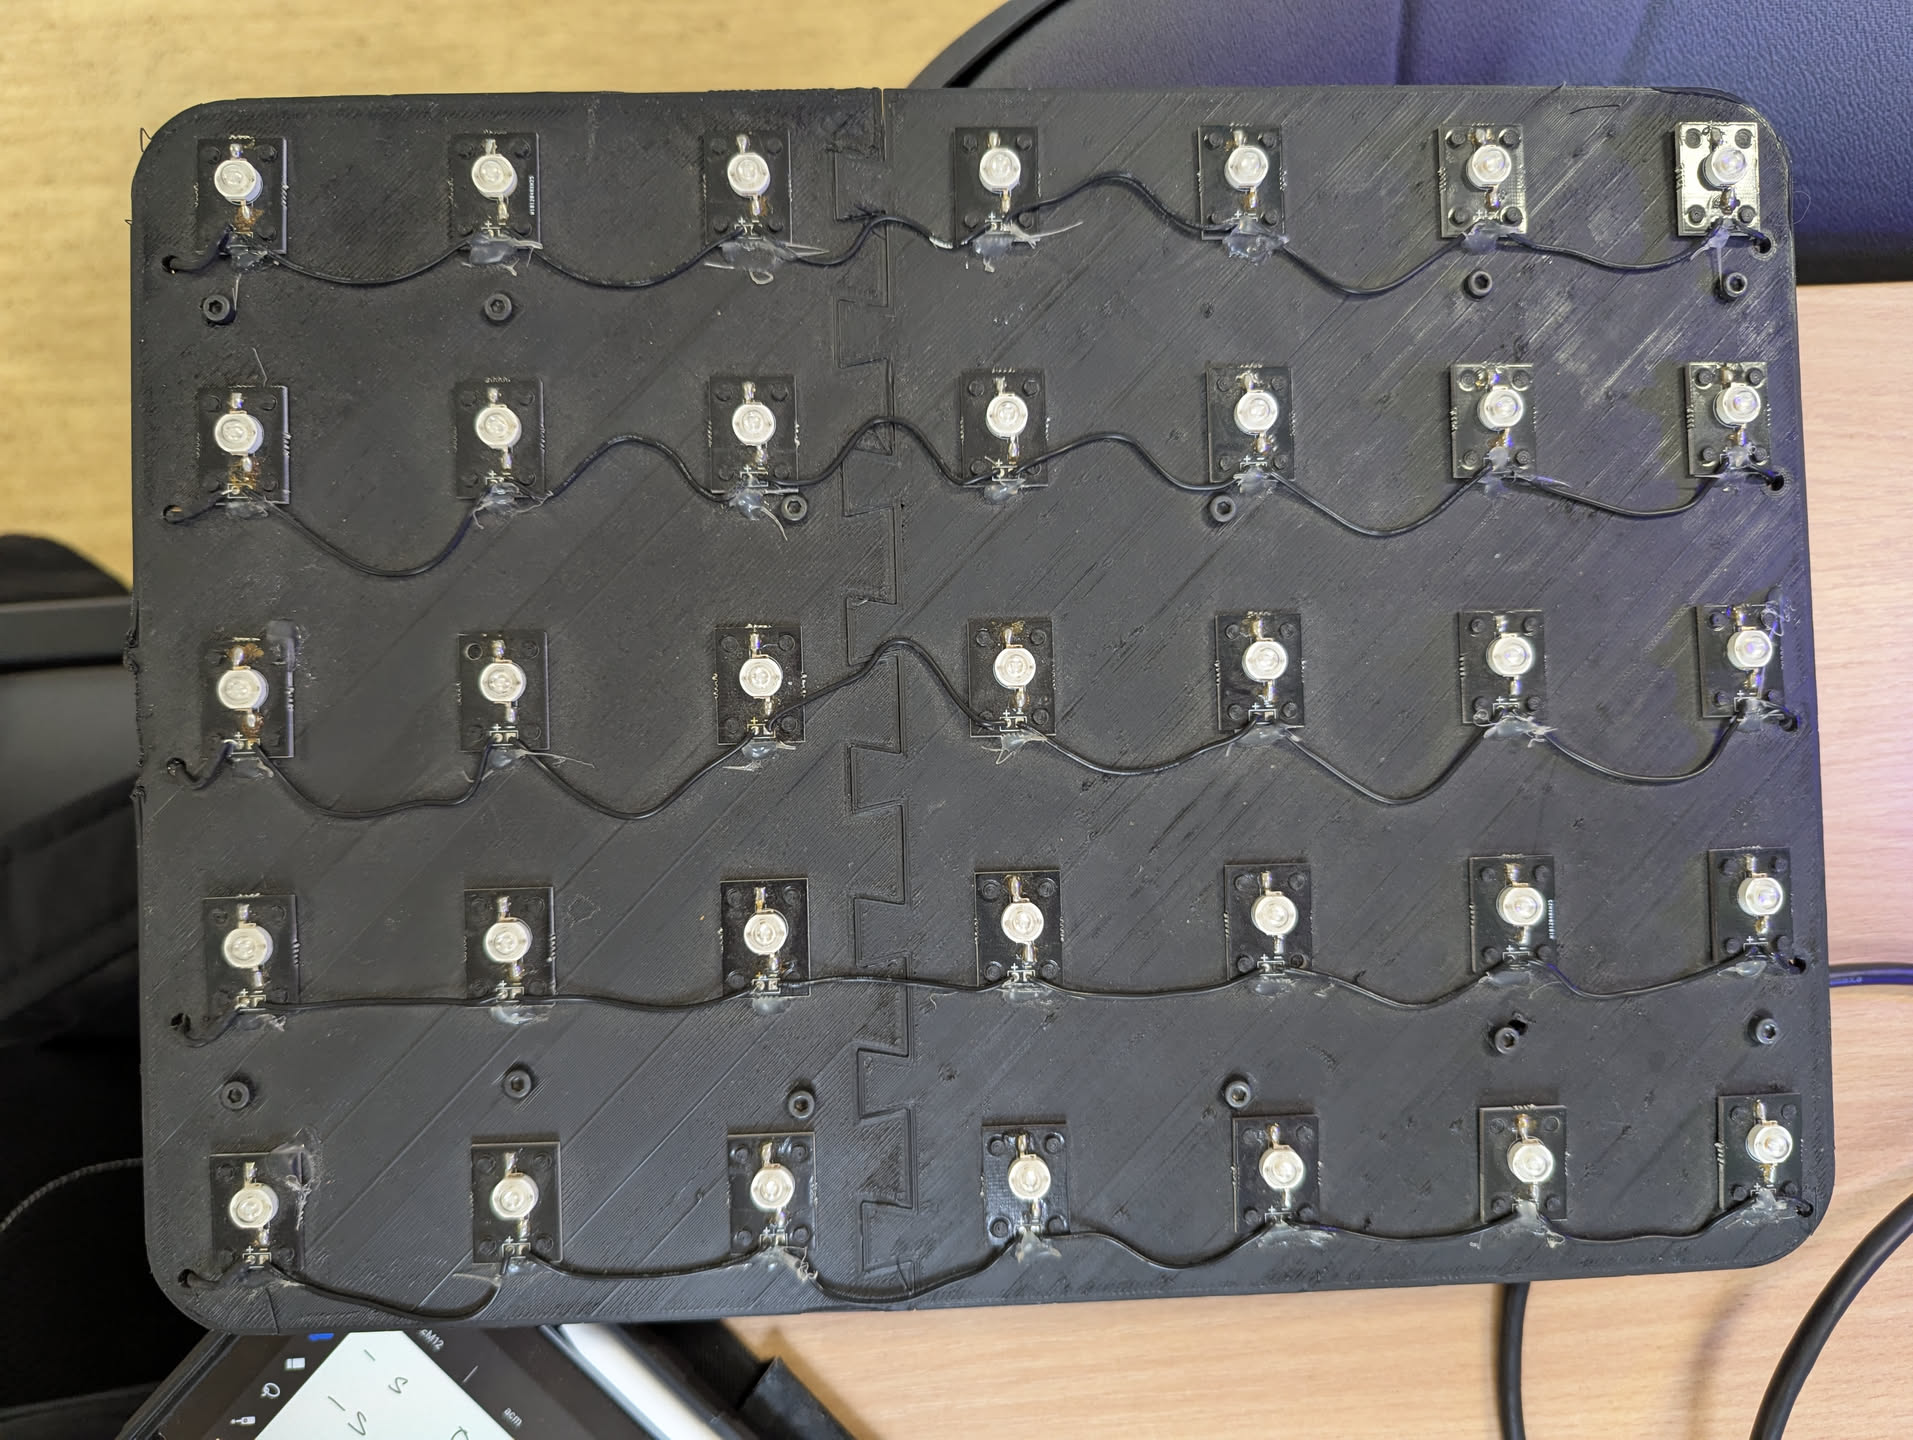
\includegraphics[width=0.5\textwidth]{./fig/photos/lattice.jpeg}
	  \label{fig:lattice_1}
	}
	\subfloat[Image from the event camera of the calibration lattice] {
	  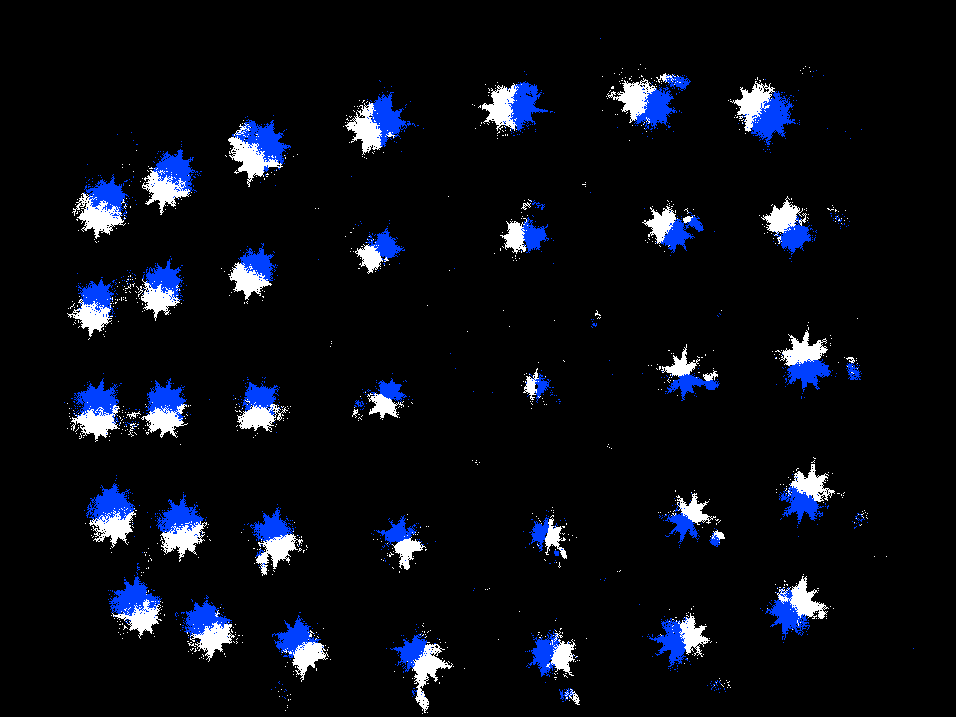
\includegraphics[width=0.5\textwidth]{./fig/photos/lattice_evs.png}
	  \label{fig:lattice_2}
	}
	\caption{
		Calibration lattice of $5\times7$ UV LEDs on \reffig{fig:lattice_1} and the events being produced when placed in front of the camera at \reffig{fig:lattice_2},
		with typical fish-eye lens distortion.
  }
	\label{fig:lattice}
\end{figure}
The downside of using an LED lattice instead of a chessboard pattern is that at a very high \ac{FOV}, the distortion of the fish eye lens sometimes does not allow
reliable detection of the exact center of the blobs (or which events correspond to which \ac{LED}), as can be seen at \reffig{fig:calibration_pattern_distorted}.
\begin{figure}[H]
  \centering
  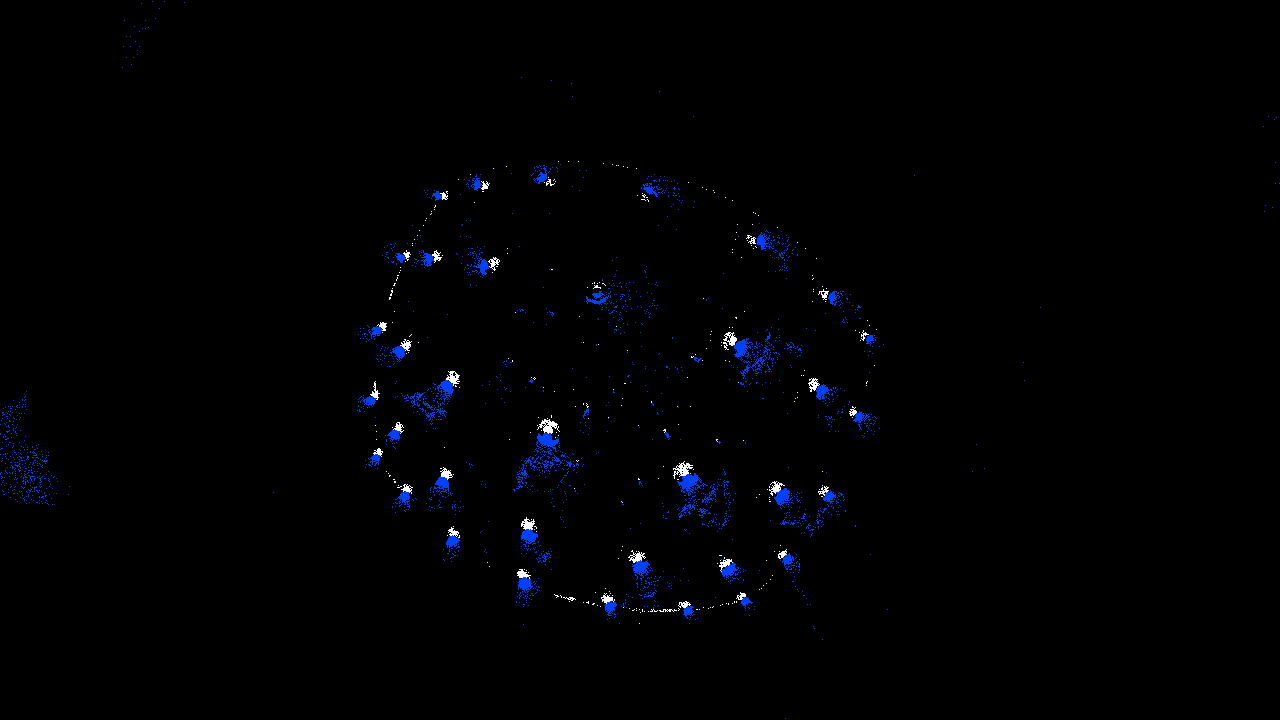
\includegraphics[width=0.7\textwidth]{./fig/photos/lattice_280.png}
  \caption{Calibration pattern with $5\times7$ lattice of UV LEDs, taken with a lens with Entaniya lens with \ac{FOV} of 280 degrees.}
  \label{fig:calibration_pattern_distorted}
\end{figure}

As we are not using a regular image of a chessboard pattern, rather a recording of accumulated events, some data preprocessing has to be done beforehand.
For the purpose of this, a simple Python app has been written. An event raw recording is loaded, and events are accumulated over a select period of time.
The accumulated events are then saved to a grayscale image, where each pixel corresponds to the number of events that occurred in that
pixel \footnote{\url{https://github.com/kubakubakuba/metavision-pyocamcalib/blob/main/generate_frames.py}}. The image is then normalized,
and the LED centers are detected using the \texttt{findContours} function of the OpenCV \footnote{\url{https://github.com/kubakubakuba/metavision-pyocamcalib/blob/main/detect_blob_centers.py}} library.
The detected centers can then be manually labeled row-wise, in the same order in every image, so the calibration process can identify 
how the grid of points changes across the images, and thus calculate the lens distortion.
After this, the regular calibration script from \texttt{py-OCamCalib} can be used with the prelabeled grid points, the labeling of the LED centers can be seen in \reffig{fig:calibration_pattern_labeled}.

\begin{figure}[H]
  \centering
  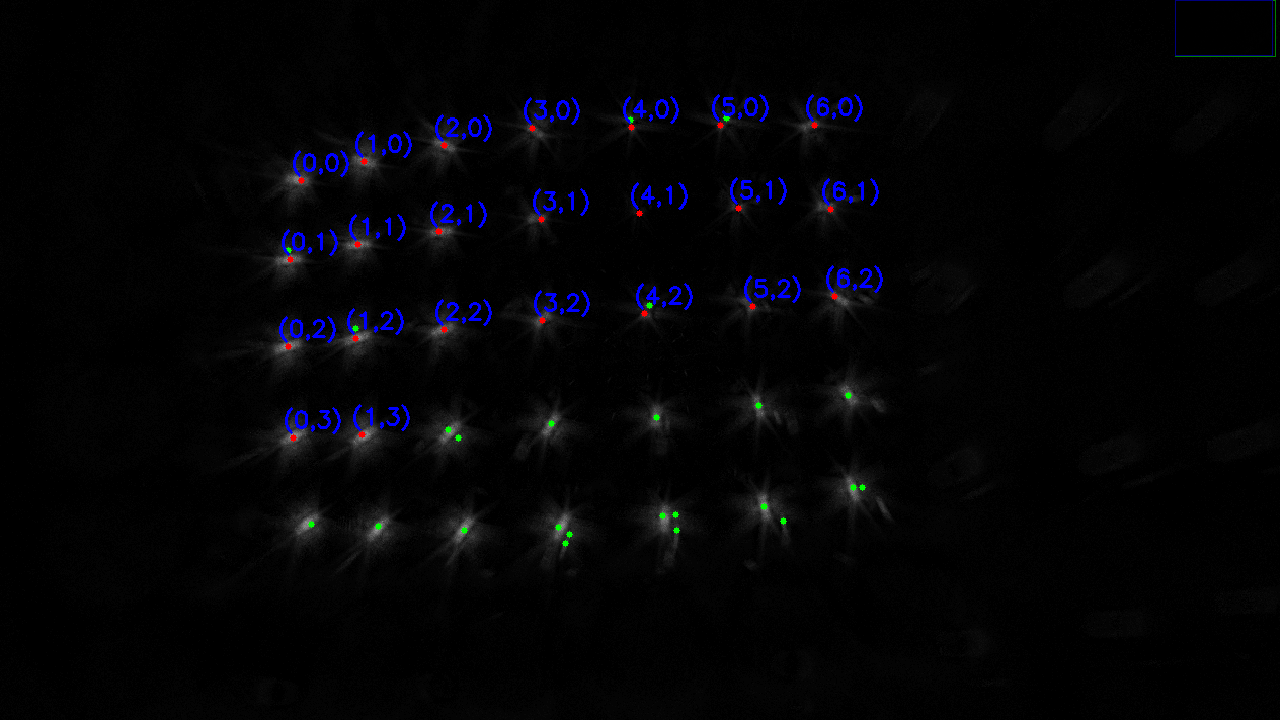
\includegraphics[width=0.7\textwidth]{./fig/photos/lattice_blobs.png}
  \caption{Calibration pattern with 5x7 lattice of UV LEDs, with the centers of the LEDs being labeled.}
  \label{fig:calibration_pattern_labeled}
\end{figure}

\section{Principles of the calibration}

After the calibration is performed, we are able to map the 3D world coordinates to the 2D image plane. For this, the calibration method needs to obtain the extrinsic
and intrinsic parameters of the camera, where the extrinsic parameters are the rotation and translation of the camera with respect to the world frame and can be expressed by equation \ref{eq:extrinsic},
\begin{equation}
	\begin{bmatrix}
		X_{camera} \\
		Y_{camera} \\
		Z_{camera}
	\end{bmatrix}
	= \mathbf{R} 
  \begin{bmatrix}
	X_{world} \\
	Y_{world} \\
	Z_{world}
  \end{bmatrix}
  + \mathbf{t}
  \label{eq:extrinsic}
\end{equation}
which is an affine transformation that uses a rotation matrix $\mathbf{R}$ and a translation vector $\mathbf{t}$. The origin of the camera's coordinate system is at the optical center,
that is, at the intersection of the optical axis from the center of the image with the image plane. This can be represented by \reffig{fig:camera_extrinsic}.

\begin{figure}[H]
  \centering
  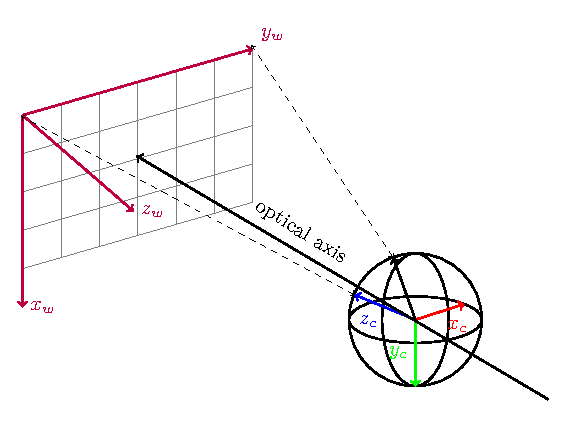
\includegraphics[width=0.7\textwidth]{./fig/tikz/extrinsic.pdf}
  \caption{Extrinsic parameters of the camera.}
  \label{fig:camera_extrinsic}
\end{figure}

The next step in the camera calibration is to fit an encompassing ellipse to the received data. The purpose of this is to see the center of distortion of the fish eye lens, as well
as the stretching of the image on both the x and y axes. This process can be seen in \reffig{fig:ellipse}. This ellipse is then used to calculate the point-mapping functions, which allows for tranformation of points from
the image plane to their respective 3D coordinates.
\begin{figure}[H]
	\centering
	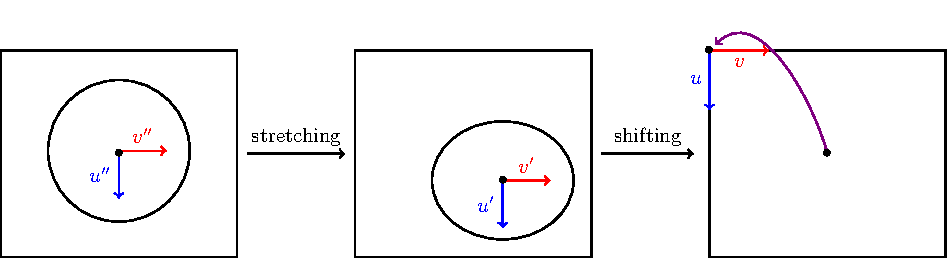
\includegraphics[width=0.9\textwidth]{./fig/tikz/ellipse.pdf}
	\caption{Encompassing ellipse fitting}
	\label{fig:ellipse}
  \end{figure}
The intrinsic parameters of the camera specify the image format itself, which is influenced by the focal length, sensor size, and optical center. As there are many mapping
functions that can be used while modeling the lens (their precision is limited by the manufacturing process), Scaramuzza et al. \cite{scaramuzzacalibration} proposed
fitting a polynomial to find the optimal model for lens calibration. The mapping functions are shown in \reffig{fig:mapping_functions}.
\begin{figure}[H]
  \centering
  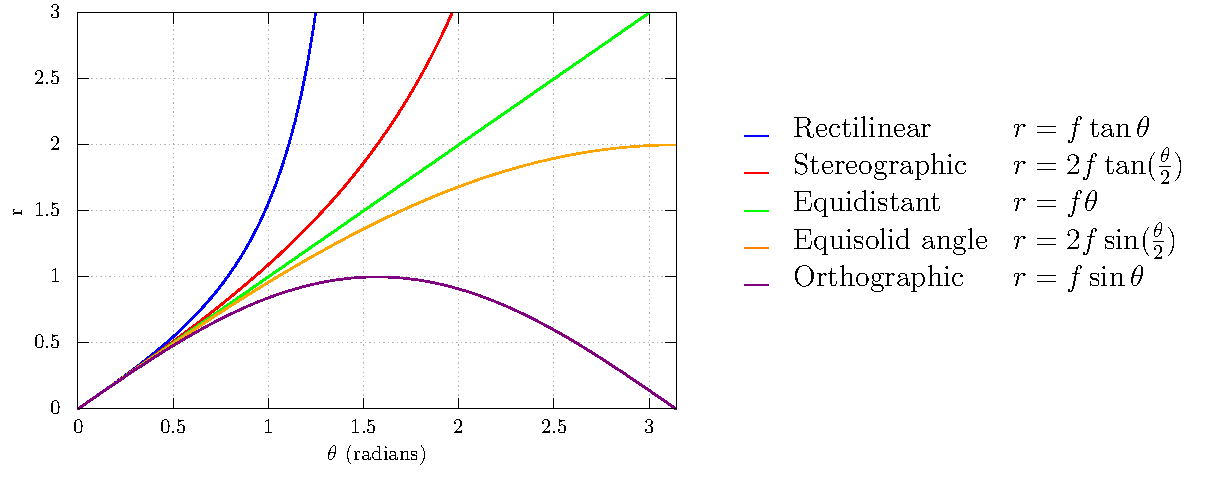
\includegraphics[width=0.9\textwidth]{./fig/tikz/mapping.pdf}
  \caption{Fisheye mapping functions, $f$ is a parameter (focal length).}
  \label{fig:mapping_functions}
\end{figure}

After we fit a polynomial, we can map the image points to their corresponding 3D vectors by an equation \ref{eq:intrinsic}.
\begin{equation}
	\lambda \cdot \alpha \cdot
	\begin{bmatrix}
		u' \\
		v' \\
		a_0 + a_1 \rho + \dots + a_{N} \rho^{N} 
	\end{bmatrix}
	= \mathbf{P} \cdot \mathbf{X_w} = %TODO: DOUBLE CHECK X_w is really the world point 
	\begin{bmatrix}
		X_c \\
		Y_c \\
		Z_c
	\end{bmatrix}
	\label{eq:intrinsic}
\end{equation}
where:

$\lambda$ is a scalar factor

$\alpha$ is a scaling factor that we obtain from \reffig{fig:ellipse} by stretching the ellipse back to a circle and performing
the affine transformation; $\alpha, \lambda > 0$

$\rho$ is the Euclidean distance of a point from the center; $\rho = \sqrt{u^2 + v^2}$

$a_0, \dots a_N$ are the polynomial coefficients and $\mathbf{P}$ is 
the perspective projection matrix.

We can also write another relation between a point $\textbf{m}' = \begin{bmatrix} u' & v' \end{bmatrix}^{T}$ in the image plane
and its corresponding point on the sensor plane $\textbf{m} = \begin{bmatrix} u & v \end{bmatrix}^{T}$. The coordinates of
$\textbf{m}'$ have the origin at the top left corner of the image, whereas the coordinates of $\textbf{m}$ have the origin in the center of the image.
This can be represented by an affine transformation $\textbf{m}' = \textbf{Am} + \textbf{O}_c$, on \ref{eq:affine} \cite{URBAN201572}.

\begin{equation}
	\begin{bmatrix}
		u' \\
		v'
	\end{bmatrix}
	= 
	\begin{bmatrix}
		c & d \\
		e & 1
	\end{bmatrix}
	\begin{bmatrix}
		u \\
		v
	\end{bmatrix}
	+
	\begin{bmatrix}
		o_u \\
		o_v
	\end{bmatrix}
\label{eq:affine}
\end{equation}

where matrix A accounts for lens-sensor misalignment, and the vector $\textbf{O}_c$ captures the relation with the center of the distortion. 

\section{Calibration results}

The camera calibration was performed on a series of images, where the calibration lattice was placed as various angles and distances from the camera.
For ideal calibration results, the lattice should be placed in all visible parts of the image, as the distortion of the fish eye is more pronounced at the edges
of the visible area. The calibration was performed on a polynomial of degree 4, more would lead to overfitting and is also not necessary.
The calibration results can be seen in \reffig{fig:calib_r}.

\begin{figure}[H]
	\centering
	\subfloat[Calibrated lens model function] {
	  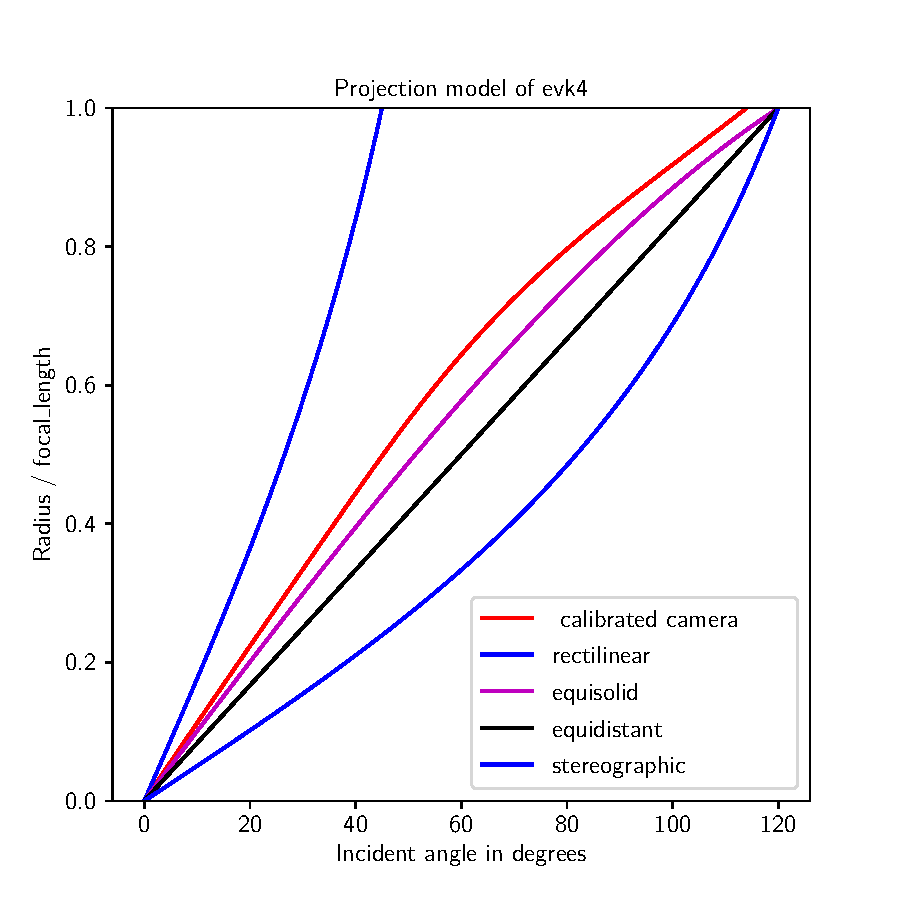
\includegraphics[width=0.45\textwidth]{./fig/pgfplot/build/evk4_projection_new.pdf}
	  \label{fig:calib_r_1}
	}
	\subfloat[Calibration images mean reprojection errors] {
	  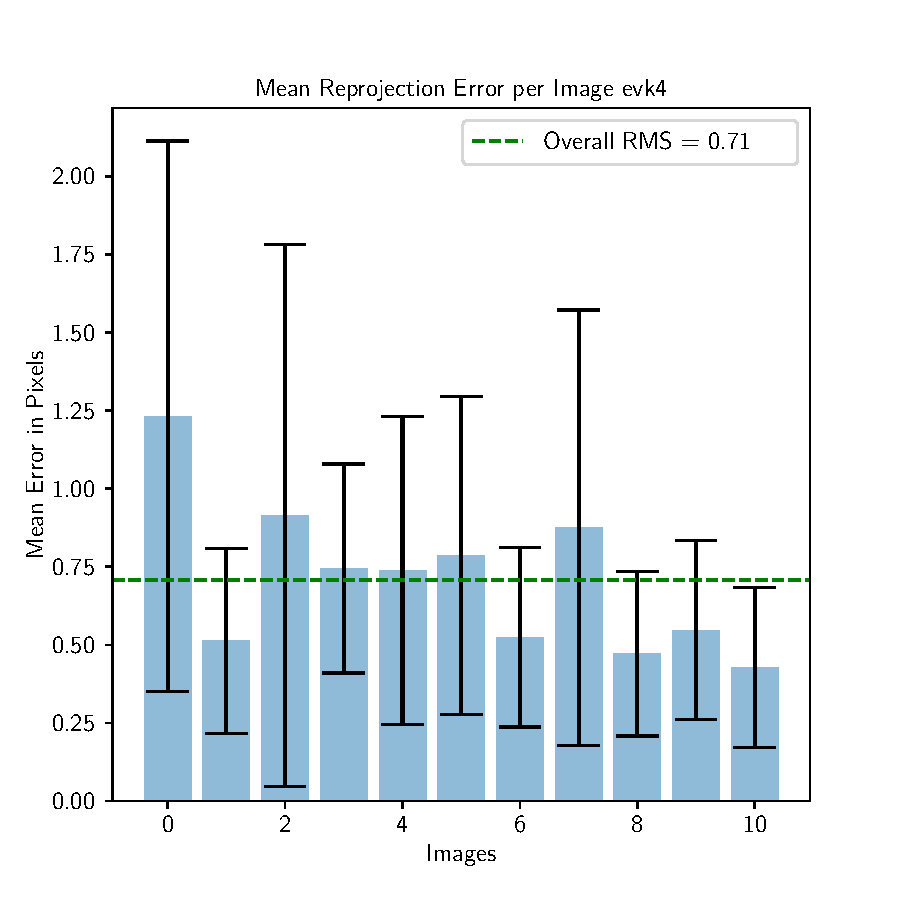
\includegraphics[width=0.45\textwidth]{./fig/pgfplot/build/evk4_reprojection_error_new.pdf}
	  \label{fig:calib_r_2}
	}
	\caption{
		Calibration results with the calibrated lens model function highlighted in red in \reffig{fig:calib_r_1} and the calibration images mean reprojection errors on \reffig{fig:calib_r_2}.
  }
	\label{fig:calib_r}
\end{figure}

The problem of fitting a minimal encompassing ellipse to event data can be formulated as an unconstrained optimization problem \ref{eq:ellipse_opt}, where we minimize the squared distances of convex hull points to the ellipse boundary.
% of minimizing the sum of point distances, that lie outside of the
%ellipse, while minimizing the ellipse parameters $a$, $b$.
The optimized ellipse can be seen in \reffig{fig:ellipse_fit}.
\begin{equation}
(a^*, b^*) = \underset{a, b > 0}{\text{argmin}} \quad \sum_{(x_i,y_i) \in \mathcal{H}} \left( \frac{x_i^2}{a^2} + \frac{y_i^2}{b^2} - 1 \right)^2
\label{eq:ellipse_opt}
\end{equation}
\text{where} $\mathcal{H} = \text{Conv}\{(x_i,y_i)\}_{i=1}^n$ is the convex hull of generated event points.

%\begin{figure}[H]
%	\centering
%	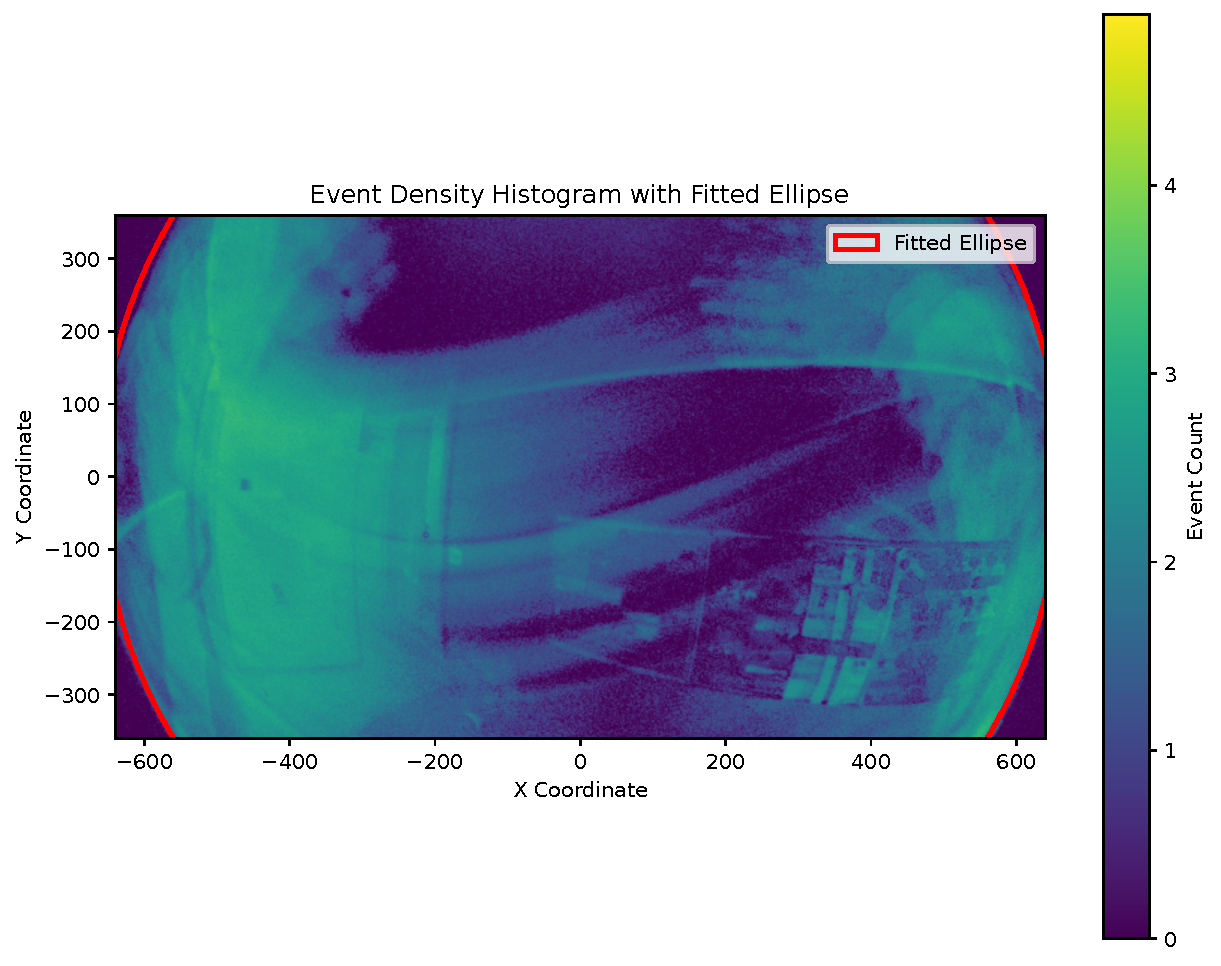
\includegraphics[width=0.65\textwidth]{./fig/svg/ellipse_fit.pdf}
%	\caption{Fitted ellipse to the calibration data, with semi-major axis $a^* = 652$, and semi-minor axis $b^* = 650$.}
%	\label{fig:ellipse_fit}
%\end{figure}
\begin{figure}[H]
	\centering
	\subfloat[Fitted ellipse.] {
	  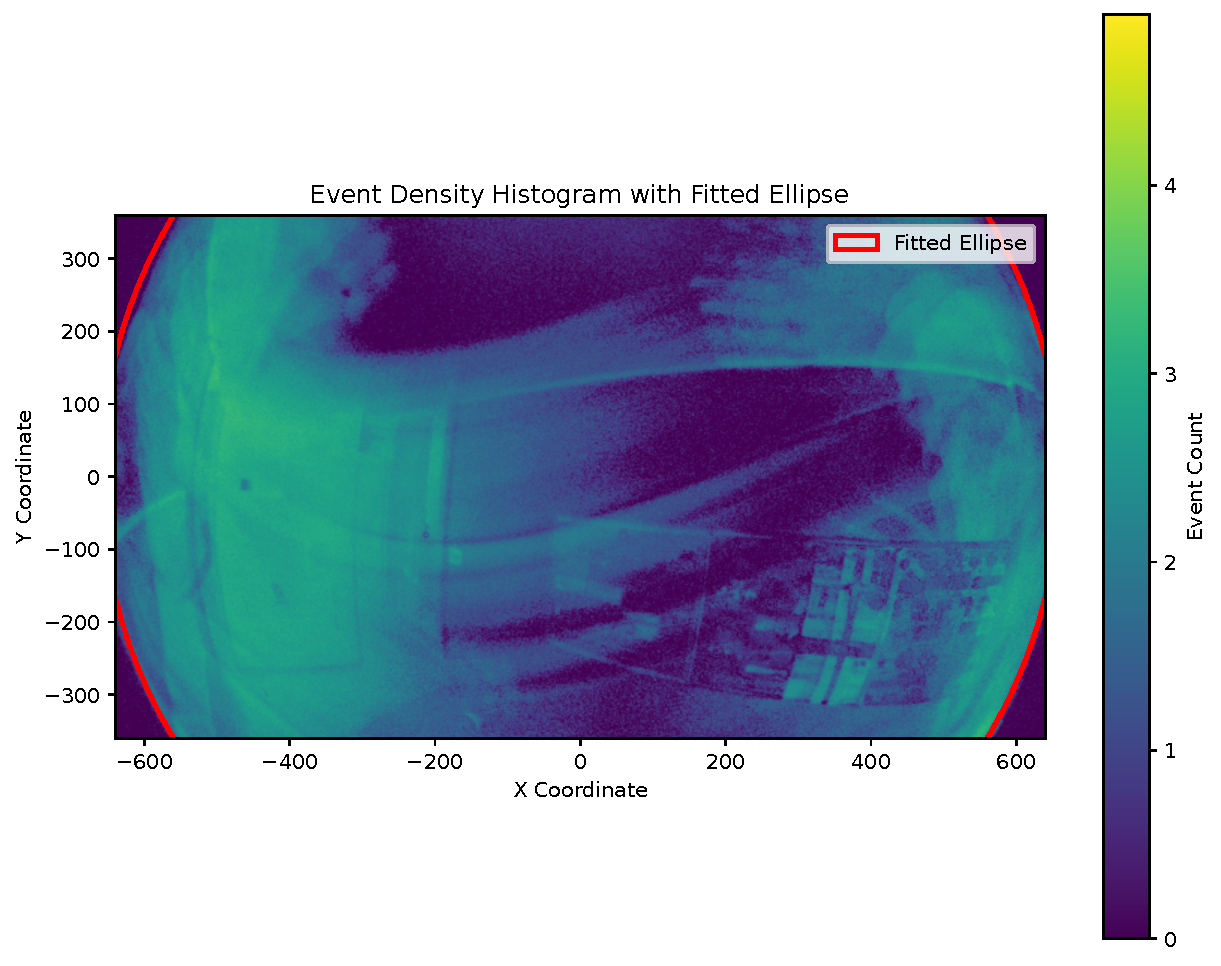
\includegraphics[width=0.5\textwidth]{./fig/svg/ellipse_fit.pdf}
	  \label{fig:ellipse_fit_1}
	}
	\subfloat[Events with convex hull points] {
	  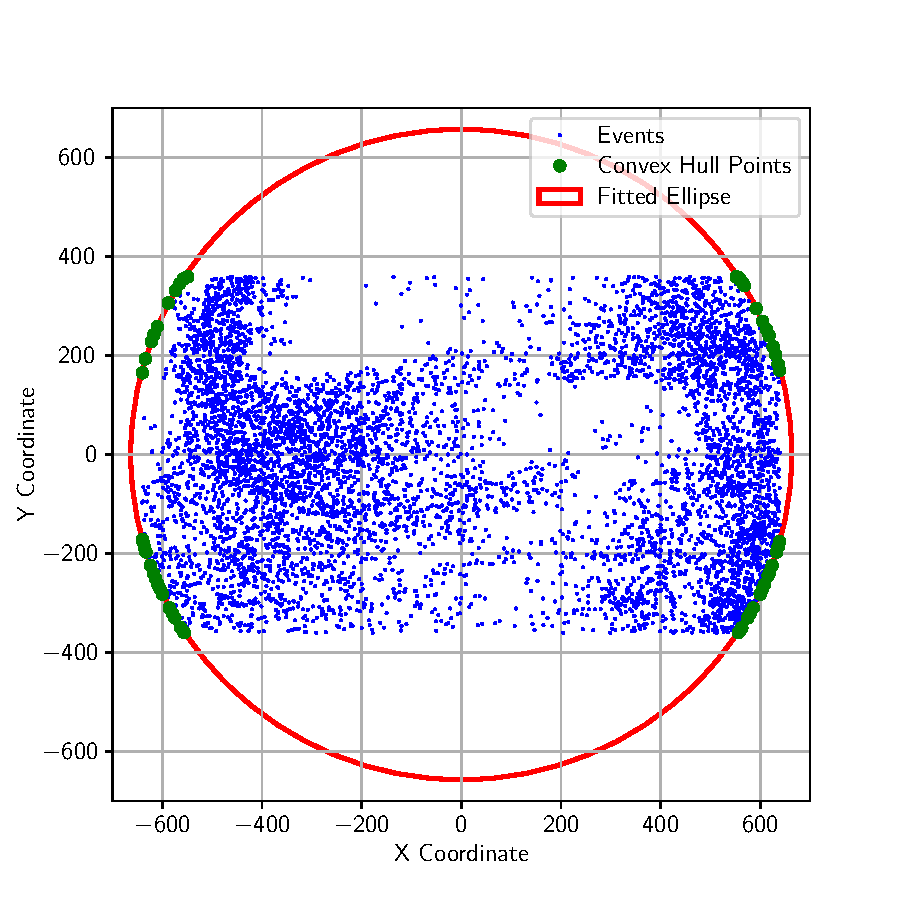
\includegraphics[width=0.45\textwidth]{./fig/pgfplot/build/ellipse_hull.pdf}
	  \label{fig:ellipse_fit_2}
	}
	\caption{
		Fitted ellipse to the calibration data, with semi-major axis $a^* = 663$, and semi-minor axis $b^* = 657$
        on \reffig{fig:ellipse_fit_1} with separated convex hull points in green on \reffig{fig:ellipse_fit_2}.
  }
	\label{fig:ellipse_fit}
\end{figure}

Finally, to visualize the calibration results, we map every point from the image plane using the \texttt{cam2world}\footnote{\url{https://github.com/jakarto3d/py-OCamCalib/blob/main/src/pyocamcalib/modelling/camera.py}}
function from py-OCamCalib, which takes a 2D image point, and returns
the corresponding 3D optical ray on the camera's unit sphere. For each point, we calculate its angle from the optical axis (a vector $\mathbf{v} = \begin{bmatrix} 0 & 0 & 1 \end{bmatrix}^{T}$),
and mask out the visible area with the ellipse fitted in \reffig{fig:ellipse_fit}. We can see the results in \reffig{fig:calibration_viz}.

\begin{figure}[H]
	\centering
	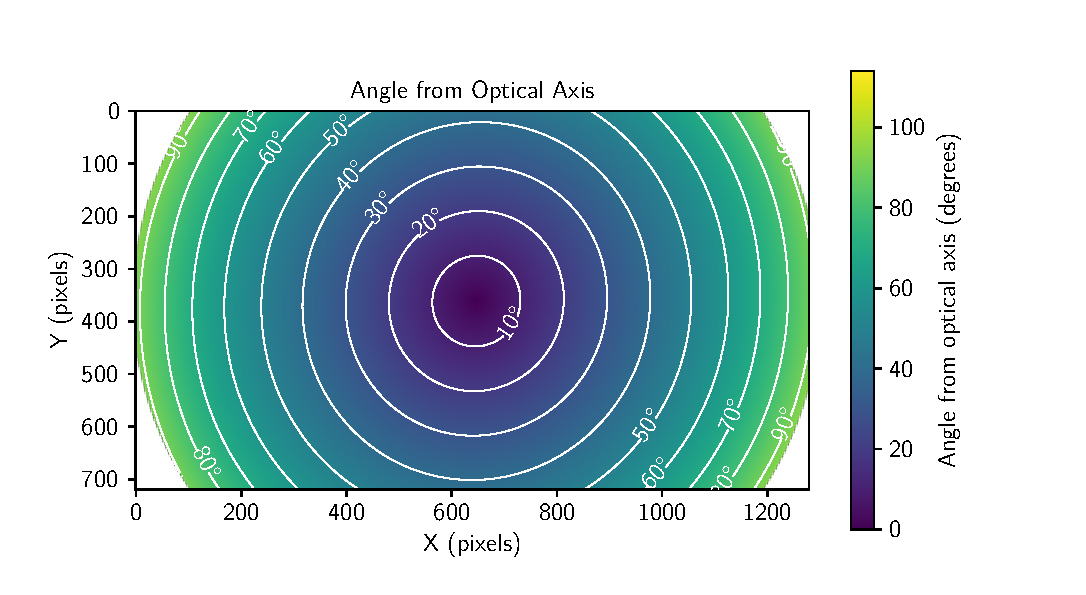
\includegraphics[width=1.0\textwidth]{./fig/pgfplot/build/evk4_viz.pdf}
	\caption{Angle from optical axis visualization, with the maximum angle of 93.47 degrees.}
	\label{fig:calibration_viz}
\end{figure}

We can also apply a perspective conversion to the whole image, which now correctly represents distances and angles. We can notice this by looking
at the calibration lattice at \reffig{fig:calib_c}, which now looks like a grid of points.

\begin{figure}[H]
	\centering
	\subfloat[Uncalibrated image.] {
	  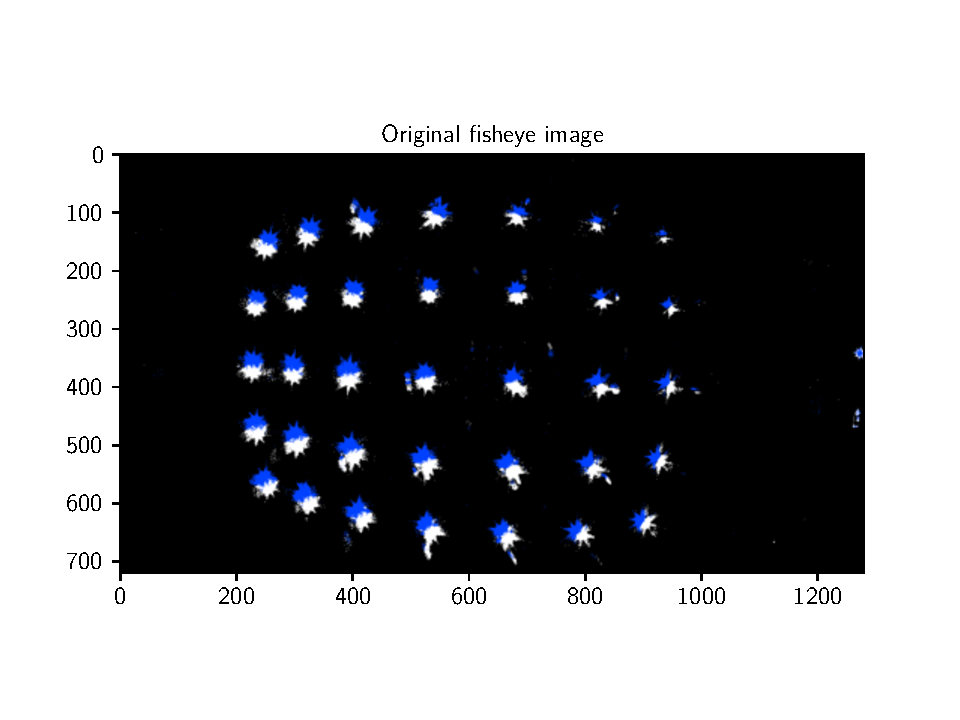
\includegraphics[width=0.5\textwidth]{./fig/pgfplot/build/image_uncalib.pdf}
	  \label{fig:calib_c_1}
	}
	\subfloat[Calibrated image.] {
	  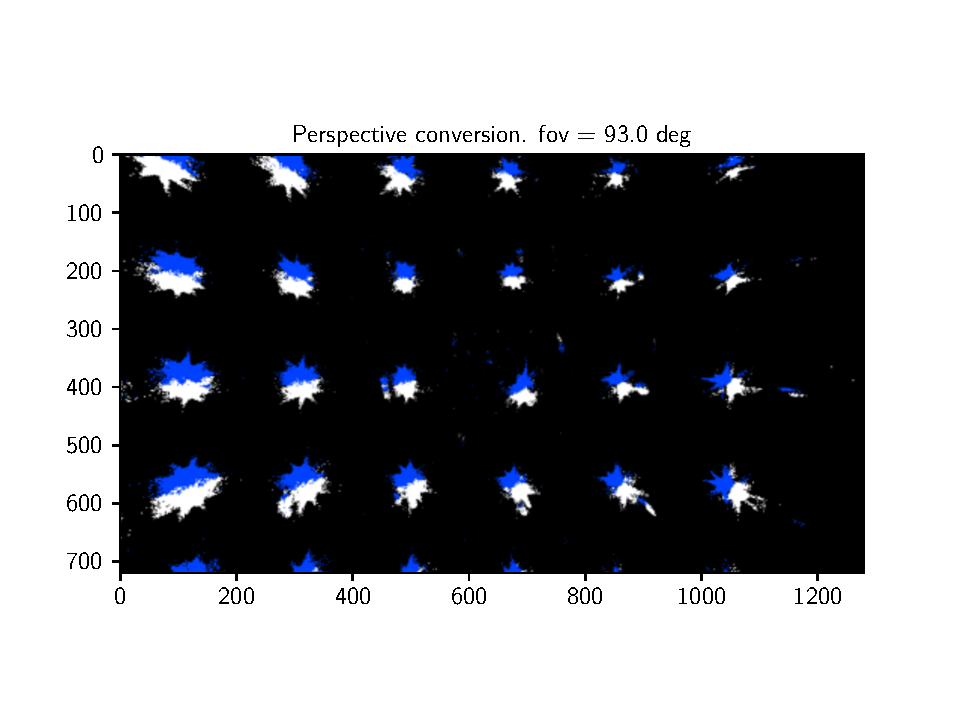
\includegraphics[width=0.5\textwidth]{./fig/pgfplot/build/image_calib.pdf}
	  \label{fig:calib_c_2}
	}
	\caption{
		Two photos of the calibration lattice, one uncalibrated on \reffig{fig:calib_c_1} and the one calibrated at \reffig{fig:calib_c_2}, which does not
		exhibit any distortion.
  }
	\label{fig:calib_c}
\end{figure}

For the calibration of the Entaniya $280$ degree lens a classical chessboard target was used, as the precise localization of the blob centers proved to be nearly impossible while using the \ac{LED} lattice calibration target. The corners of the chessboard pattern provide
better contrast and allow for precise localization of the center; unfortunately, they need to be labeled manually in this case as seen in \reffig{fig:calib_ent_label}.
The calibration results can be seen on \reffig{fig:calib_e}, with the visualization on \reffig{fig:calib_ent_viz} and the perspective projection on
\reffig{fig:calib_ent_proj}.
\begin{figure}[htbp]
	\centering
	%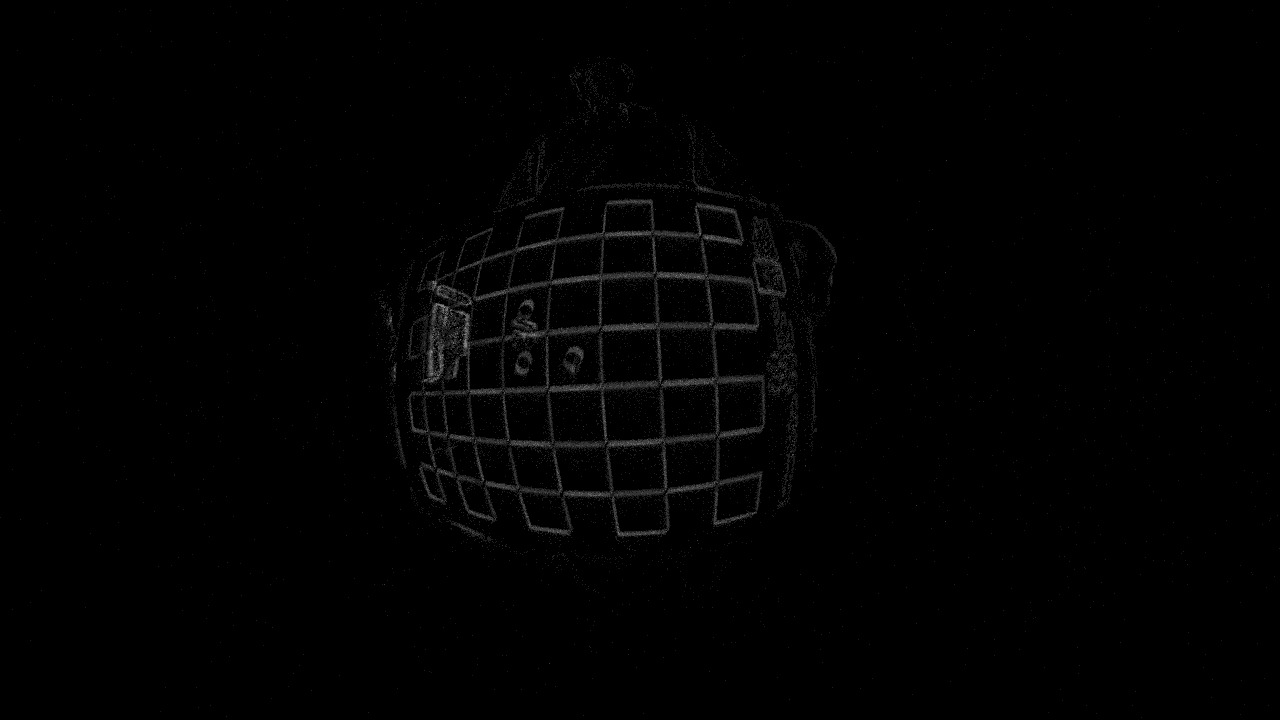
\includegraphics[width=0.6\textwidth]{./fig/photos/frame_58CEE7E0.png}
        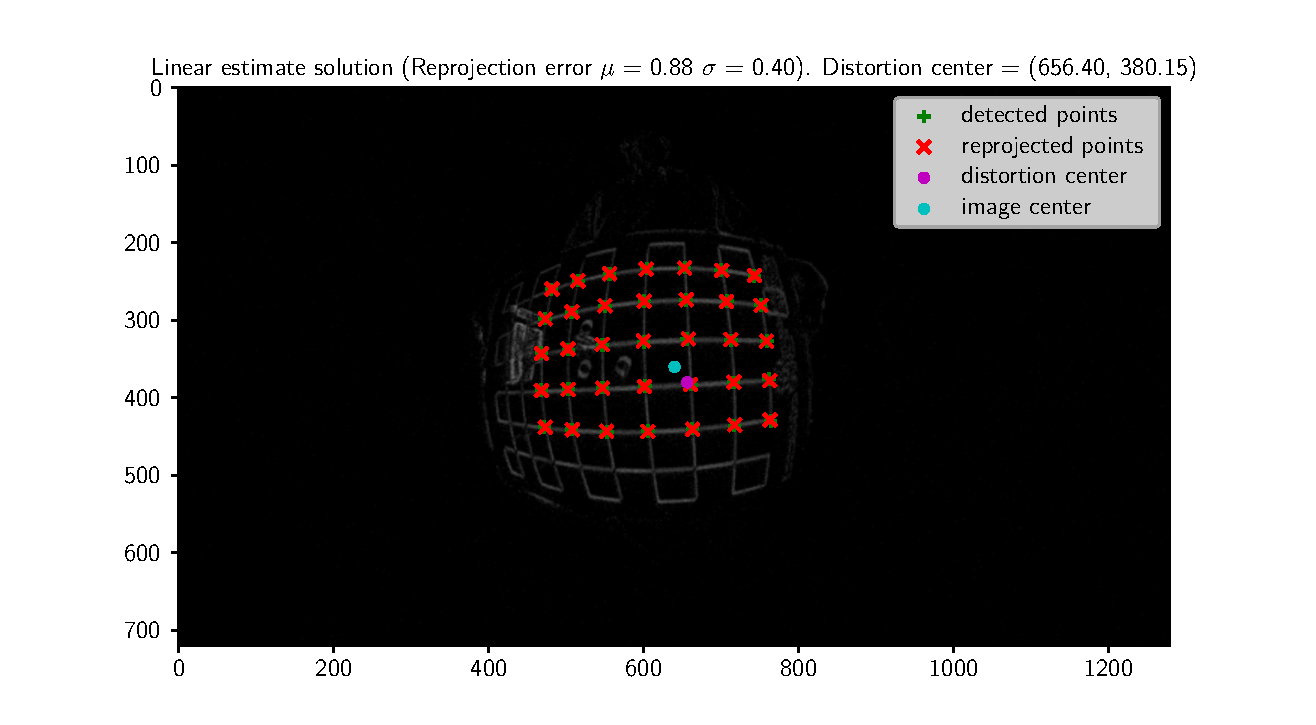
\includegraphics[width=0.8\textwidth]{./fig/pgfplot/build/chessboard_280.pdf}
	\caption{Chessboard calibration target visible in 280 degree lens with marked chessboard edge points}
	\label{fig:calib_ent_label}
\end{figure}

\begin{figure}[H]
	\centering
	\subfloat[Calibrated lens model function] {
	  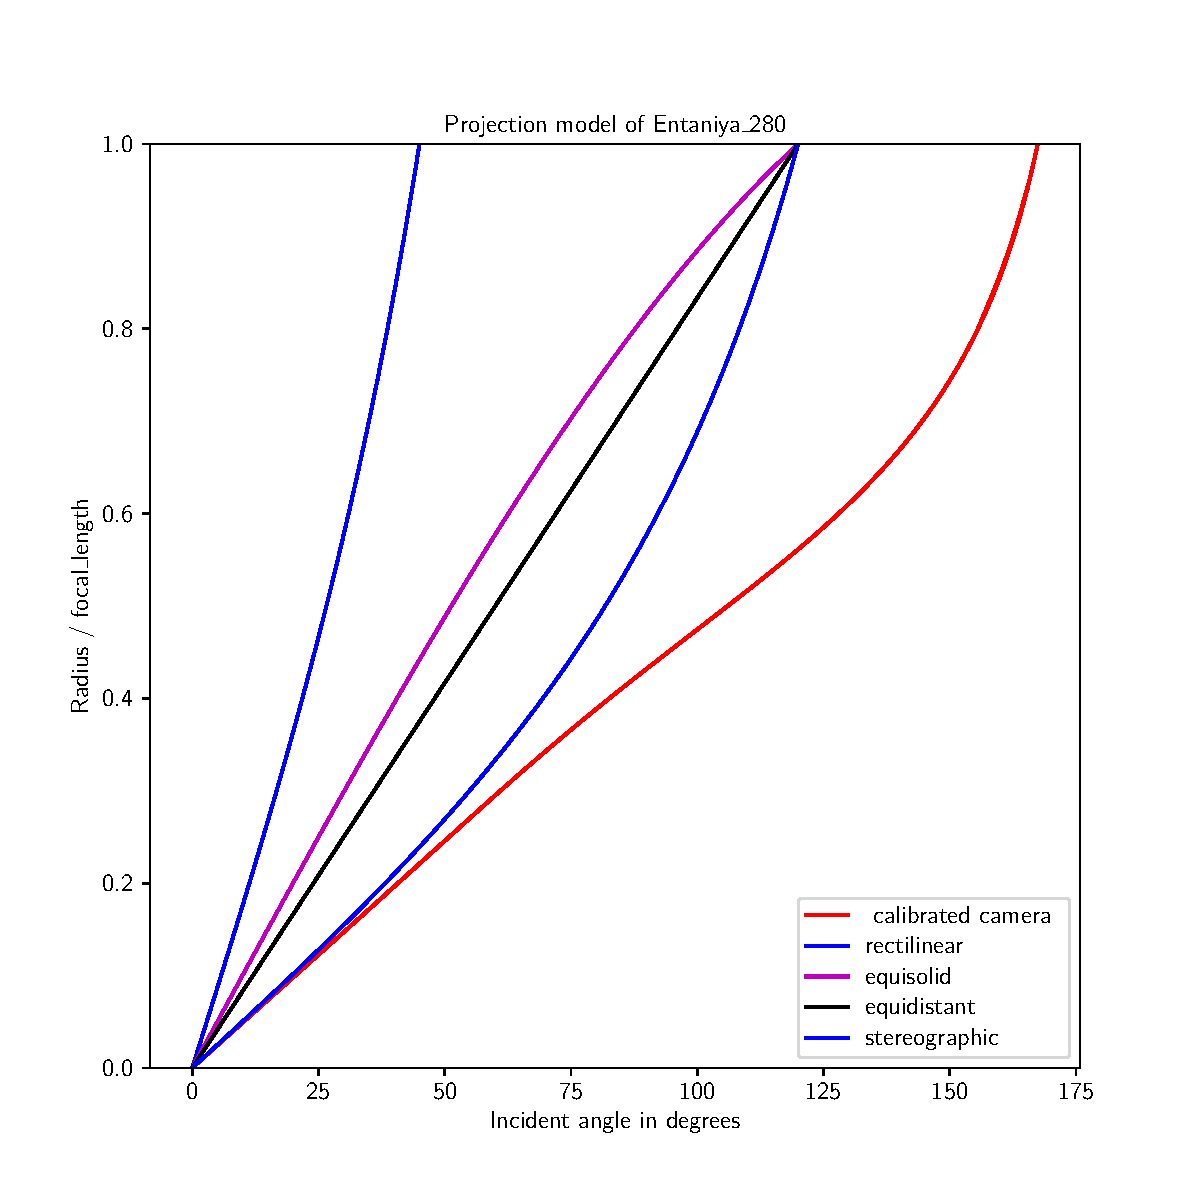
\includegraphics[width=0.5\textwidth]{./fig/pgfplot/build/proj_280_new.pdf}
	  \label{fig:calib_e_1}
	}
	\subfloat[Calibration images mean reprojection errors] {
	  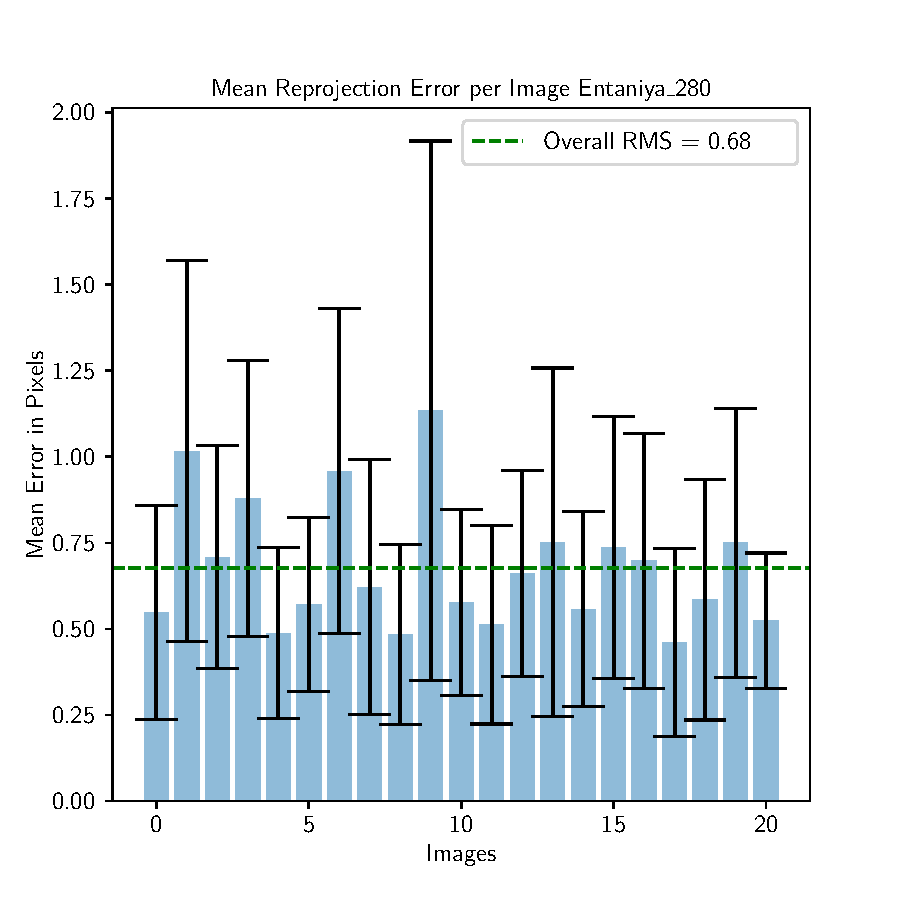
\includegraphics[width=0.5\textwidth]{./fig/pgfplot/build/err_280_new.pdf}
	  \label{fig:calib_e_2}
	}
	\caption{
		Calibration results for the Entaniya 280 degree lens with the calibrated lens model function highlighted in red in \reffig{fig:calib_e_1} and the calibration images mean reprojection errors on \reffig{fig:calib_e_2}.
  }
	\label{fig:calib_e}
\end{figure}
\begin{figure}[H]
	\centering
	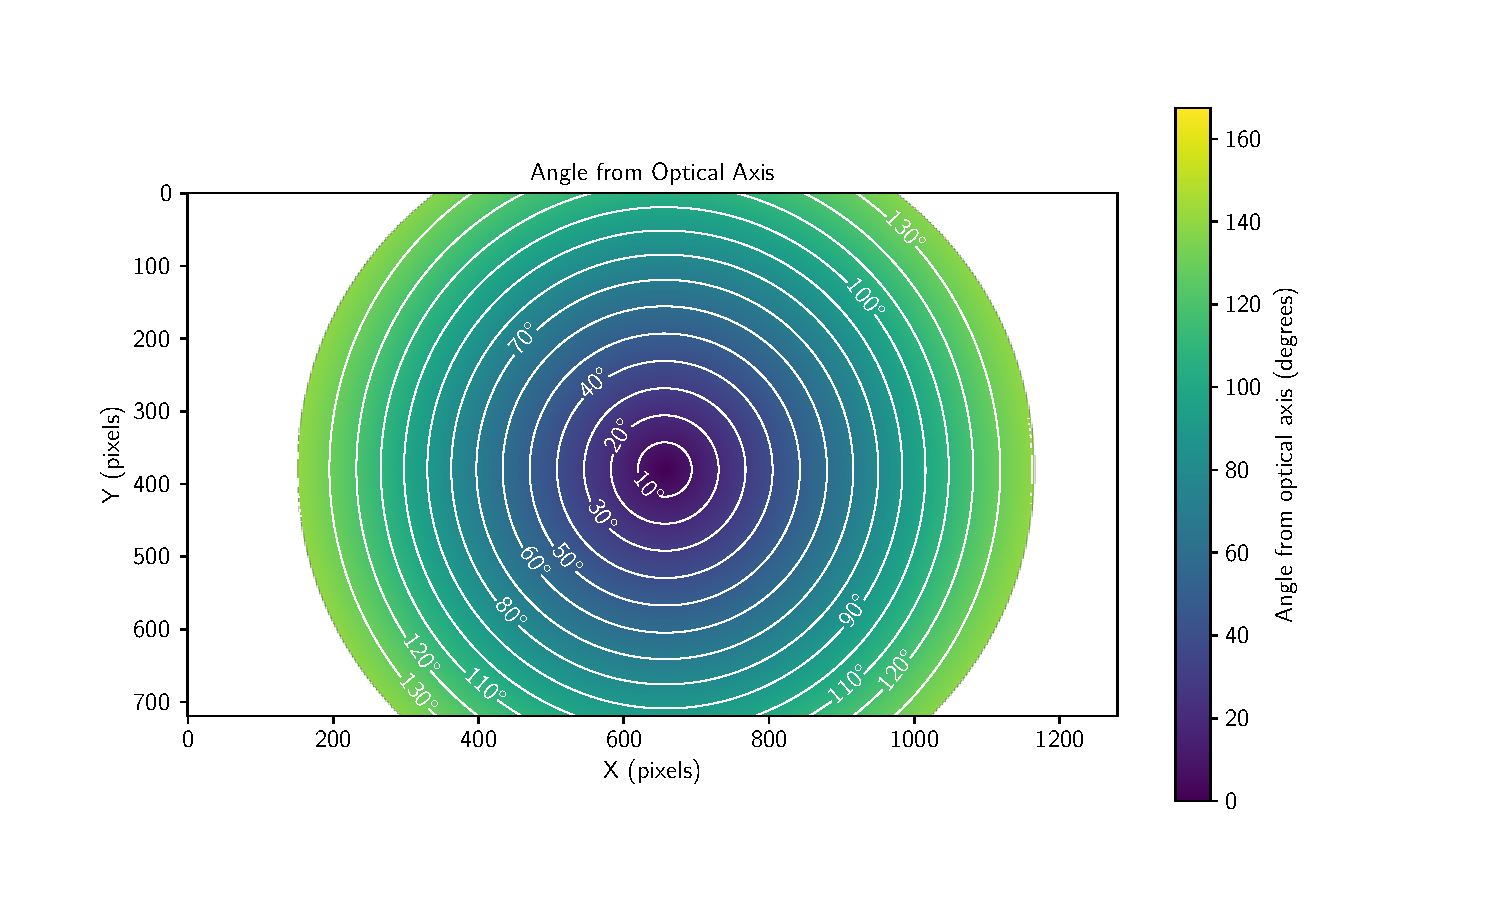
\includegraphics[width=1.0\textwidth]{./fig/pgfplot/build/viz_ent.pdf}
	\caption{Angle from optical axis visualization, with the maximum angle of 140 degrees on each side, making its \ac{FOV} 280 degrees.}
	\label{fig:calib_ent_viz}
\end{figure}
\begin{figure}[H]
	\centering
	\subfloat[Uncalibrated image.] {
	  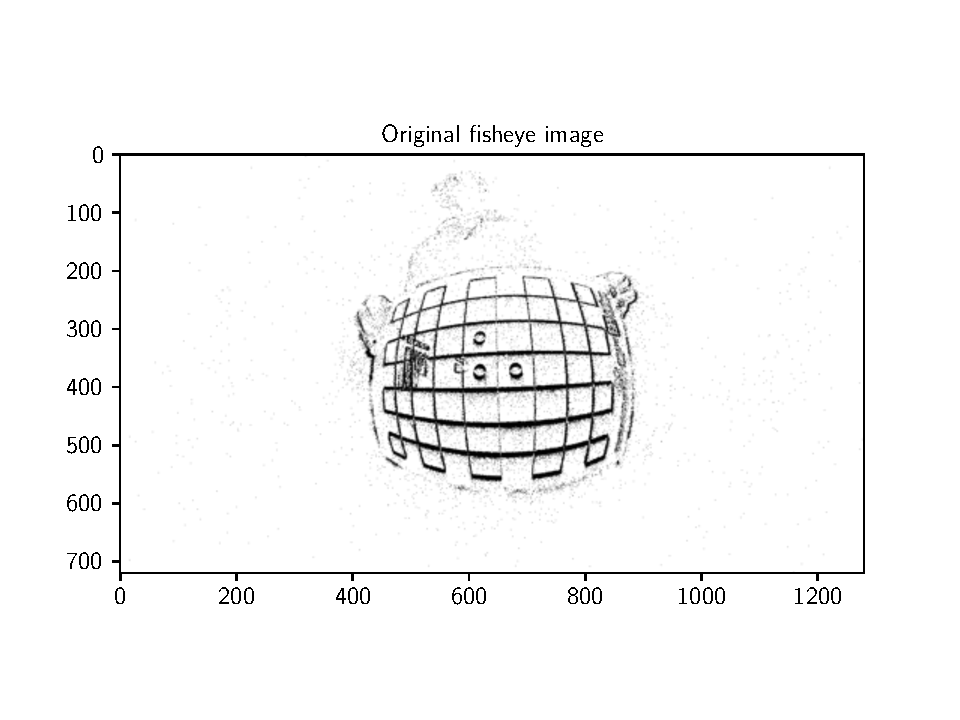
\includegraphics[width=0.5\textwidth]{./fig/pgfplot/build/ent_before.pdf}
	  \label{fig:calib_ent_proj_1}
	}
	\subfloat[Calibrated image.] {
	  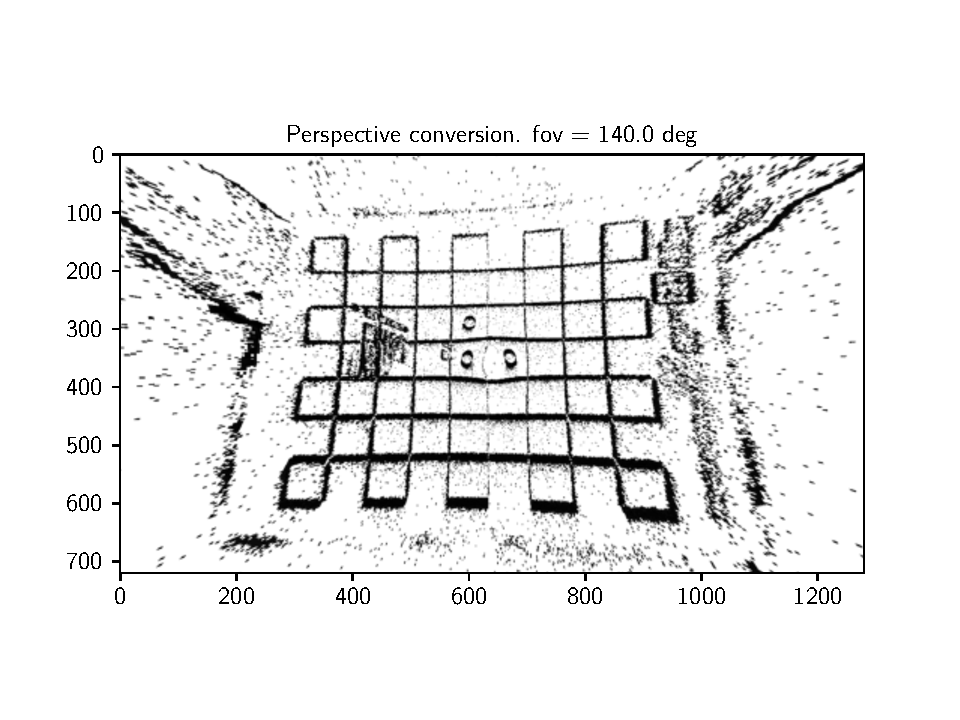
\includegraphics[width=0.5\textwidth]{./fig/pgfplot/build/ent_after.pdf}
	  \label{fig:calib_ent_proj_2}
	}
	\caption{
		Two photos of the calibration chessboard from the Entaniya 280 degree lens, one uncalibrated on \reffig{fig:calib_ent_proj_1} and the one calibrated at \reffig{fig:calib_ent_proj_1}.
  }
	\label{fig:calib_ent_proj}
\end{figure}

%\todo{change wording regarding lens FOV - inconsistent between 187 and 280 degrees (one is not the whole FOV but is mentioned as}